After cutting the licenceplate we apply some preprocessing method with OpenCV-python:
\begin{itemize}
    \item \emph{Normalization:} For normalization we used a formula that we found on the internet \url{https://nextgeninvent.com/7-steps-of-image-pre-processing-to-improve-ocr-using-python/}.
    \item \emph{Noise removal:} For the noise removal we used the 'fastNlMeansDenoisingColored' function of OpenCV.
    \item \emph{Erodation:} For the erosion's kernel we used a 5x5 matrix of ones.
    \item \emph{Blur clarification:} For the blur clarification we used a matrix with a value 9 center surrounded with -1 values.
    \item \emph{Adaptive Threshold:} For this we used the 'adaptiveThreshold' function of OpenCV
\end{itemize}

This results a much better image for the OCR. It convert the image to binary and try to sharpen the label of the licenceplate. 

\begin{align}
Blur clarification kernel &= \begin{bmatrix}
    -1, -1, -1\\
    -1, 9, -1 \\
    -1, -1, -1
\end{bmatrix}
\end{align}

\begin{figure}
    \begin{subfigure}[b]{.45\textwidth}
        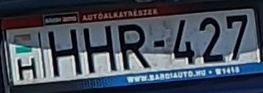
\includegraphics[width=\textwidth]{figures/preprocessbefore.jpg}
    \end{subfigure}
    \hfill
    \begin{subfigure}[b]{.45\textwidth}
        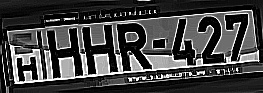
\includegraphics[width=\textwidth]{figures/preprocessafter.jpg}
    \end{subfigure}
    \hfill
    \caption{Example for preprocessing (HHR-427)}
    \label{fig:preprocessing-fig}
\end{figure}